\chapter{Funzioni di variabile complessa}

Una funzione $f:D\subset \C \to \C$ è una mappa che manda una variabile $z=x+iy$ in  $w=u+iv$, con $u$ e $v$ che sono funzioni di $x$ e $y$.

Sia ad esempio $f(z)=az$ , con $a \in \C$; essa rappresenta una mappa $z \mapsto w= |a|e^{i\alpha} |z|e^{i \, arg(z)}$; invece una funzione $f(z)=az+b$ opera nella seguente maniera:

\begin{figure}[h!]
    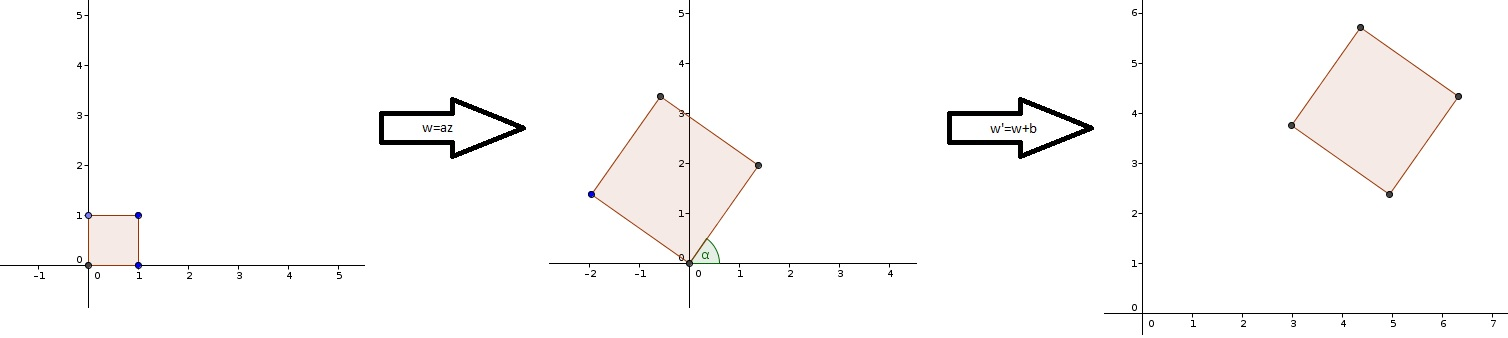
\includegraphics[width=1\textwidth]{immagini/trasformazione.jpg}
\end{figure}
Questo gruppo di trasformazioni è il gruppo delle rototraslazioni nel piano.

Prendiamo ora in considerazione la trasformazione $f(z)=z^2$ e vediamo come opera su una circonferenza:  notiamo che, se prendessimo tutta la circonferenza, otterremmo che la funzione ricopre due volte il piano complesso; per tale motivo, limitiamo il nostro dominio (ad esempio prendendo $Re(z)>0$). Presa la circonferenza di raggio unitario (centrata nell'origine), abbiamo che essa viene mandata nuovamente nella circonferenza di raggio unitario; invece le altre circonferenze centrate nell'origine vengono dilatate $(R>1)$ o ristrette $(R<1)$, mentre, come detto prima, si ha che da un semipiano complesso passiamo all'intero piano complesso.

Questo fatto può essere mostrato anche vedendo il risultato della trasformazione applicata al reticolo coordinato; infatti, abbiamo che:
$$w=z^2=(x+iy)^2=(x^2 -y^2)+2ixy=u+iv$$
A questo punto, ponendo $x$ o $y$ costanti, si ricavano le equazioni del reticolo corrispondente nel piano di arrivo che sarà formato da parabole ad asse orizzontale, con concavità rispetivamente verso sinistra ($x=cost$) e verso destra ($y=cost$).

\begin{figure}[h!]
  \centering
    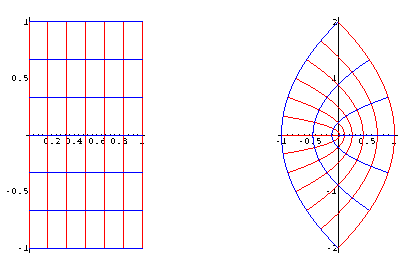
\includegraphics[width=0.4 \textwidth]{immagini/quadrato.png}
\end{figure}

Possiamo ragionare alla stessa maniera anche nel caso opposto, cioè considerando la trasformazione $f(z)=\sqrt{z}$; in questo caso, otteniamo delle iperboli.

\begin{figure}[h!]
  \centering
    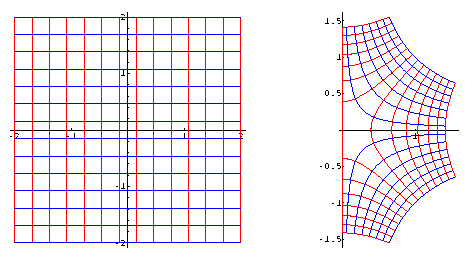
\includegraphics[width=0.4\textwidth]{immagini/quadrattto.png}
\end{figure}

In entrambi i casi, la perpendicolarità fra le linee dei reticoli coordinati viene conservata dalle trasformazioni prese in considerazione, cioè le linee perpendicolari nel piano di partenza lo sono anche nel piano di arrivo.

Infine, vediamo come la trasformazione $f(x)=\frac{1}{z}$ opera sul reticolo coordinato; abbiamo che, se $z=x+iy$, allora:
$$\frac{1}{z}=\frac{1}{x+iy}$$
Quindi, ponendoci sulle linee del reticolo coordinato, otteniamo che per $x$ o $y$ che tendono a $\infty$ la funzione tende a 0, cioè le linee si chiudono in circonferenze centrate su un punto degli assi ($\frac{1}{2x}$ o $ \frac{1}{2iy}$) e  passanti per l'origine.

\begin{figure}[h!]
  \centering
    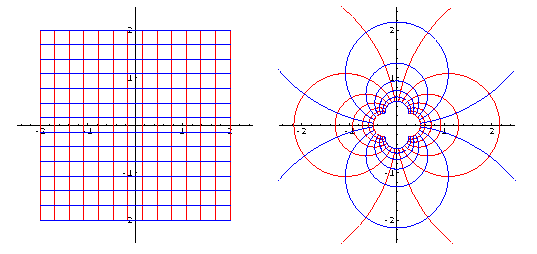
\includegraphics[width=0.4\textwidth]{immagini/inverso.png}
\end{figure}
